\graphicspath{{chapters/TumorEvStudiesIIImages/}}

The graph in the figure below puts in relation the copy number status (log2 ratio)
and the purity/clonality of the sample (Beta); the more we go towards the left
the fewer number of copies, the lower on the y axis the higher the clonality.

The best proxy of the quantity of tumor content present in a sample is done
using the lowest cluster.

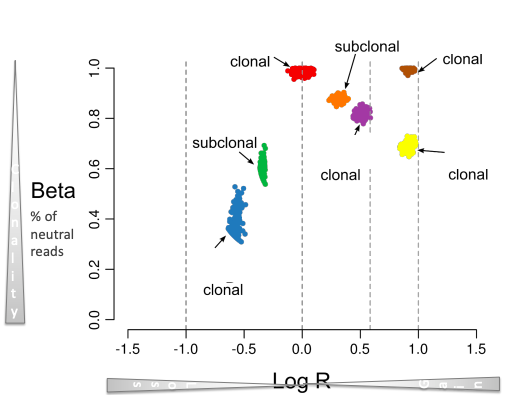
\includegraphics[width=3.46875in,height=2.65139in]{image2.png}\\



\chapter{Tumor evolution studies (continued)}

\textbf{\textit{Written by Giorgia Bucciarelli}}\\

\section{Tumor mapping}

Regarding the image presented here below:
\begin{itemize}
\item
  The \textbf{blue} cluster with deletions is the most clonal one since $\beta \sim 0$
\item
  Both \textbf{blue} and \textbf{green} clusters had deletions, since they have a negative log2
  ratio, but the green ones are less clonal than the blue ones.
\item
  In log2 R = 0 and ß = 1, where there's the \textbf{red} cluster, we have a status of no
  copy number changes (wild-type status in terms of copy numbers). This
  basically represents a total number of alleles which is the same in both the
  tumor and normal sample.
\item
  All the other clusters with a positive log2 ratio had a gain of DNA
\end{itemize}

\begin{figure}[H]
  \caption{Presence of multiple populations in the sample}
  \centering
  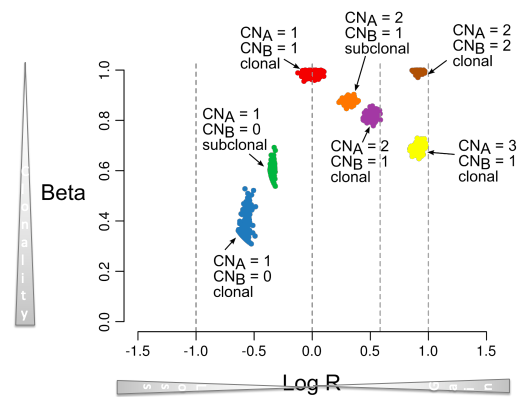
\includegraphics[width=0.8\textwidth]{image3}
  \label{fig: }
\end{figure}

In this figure the number of copies that correspond to all the clusters in the
space is also reported. \\

Analysis of different samples could be done to assess Clonality and build \emph{\textbf{evolution maps}}.

\begin{figure}[ht]
  \caption{Ordering of aberrations}
  \centering
  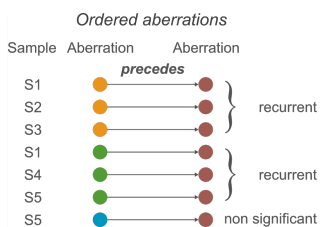
\includegraphics[width=0.7\textwidth]{image4}
  % \label{fig: ordered aberrations}
\end{figure}

In the figure:
% #TODO come mai si parla sempre di deletion?
\begin{itemize}
\item
  In sample 1 the brown lesion is subclonal to the orange one, and that same
  lesion is also subclonal to the green one.
\item
  In sample 2 we have again the support of the relation between the brown and
  orange lesion with the same level of subclonality (brown subclonal to orange).
\item
  In sample 3 is the same as in sample 1 and 2.
\item
  Samples 4 and 5 have the same clonal modification green to brown.
\item
  In sample 5 only we also have another concomitant lesion (blue subclonal to
  brown).
\end{itemize}

So we perform this analysis for all the concomitant lesions in our sample and we
start drawing the arrows to keep track of what is subclonal to what. We compile
this list across all individuals and look for how many times we see support for
the same relationship in the same direction. In our case we can say that the relationship going \textbf{from orange to brown is
supported by 3 out of 5 samples}; the same can be said for the green going to
brown. The blue one is instead not significant since it's supported by only one
individual.

\begin{figure}[H]
  \caption{evolution map. The orange and the green which have no relationship between them, are at the
  same level on the x axis in the path and they both go into brown.}
  \centering
  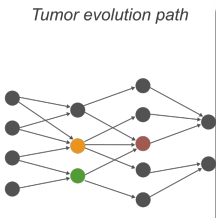
\includegraphics[width=0.5\textwidth]{image5}
  % \label{fig: }
\end{figure}



So one can assume that the more clonal a lesion is the more likely it is that it
occurred earlier during the evolution (time is on the x axis of the path), and
we can look for recurrent relationships among lesions.
Alterations could be fought in a \textit{\textbf{temporal sequence}}, following the x axis.

\begin{figure}[H]
  \caption{Prostate cancer analysis of dependencies}
  \centering
  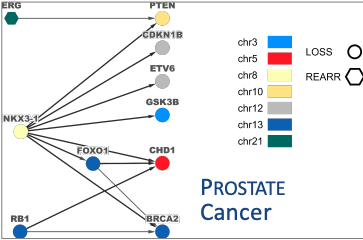
\includegraphics[width=0.6\textwidth]{image6}
  \label{fig: prostate cancer}
\end{figure}

If we do that in
large datasets (lung cancer melanoma, prostate cancer \ldots) we can come up
with all the \textbf{dependencies} that were observed and that were supported by more
than one individual (e.g. in prostate cancer we can say that a loss in NKX3-1
precedes the deletion of PTEN; figure \ref*{fig: prostate cancer}).\\

Even if we have hundreds of BAM files on whole exon sequencing data from large
collections all that we can build are \textbf{evolution maps with at most three layers}
(pretty disappointing). This has multiple reasons, one of them is that:

\begin{center}
  To build a relationship which is statistically significant between two genes
  we need to have\textbf{ multiple instances of that relationship (in many samples)}.  
\end{center}

Therefore we are tremendously limited by co-occurrence of lesions.

To boost the reconstruction of these paths \textbf{gene families or pathways} have been
exploited. \textit{\textbf{E.g.}} if we are dealing with PTEN which is a tumor-suppressive gene relevant in a
specific pathway (PF3K), then it doesn't matter if we have deletion or
inactivation of the same genes in the same pathway, what matters for the tumor
evolution is that that specific pathway is altered and so what we can do is
start aggregating signals.\\

With this method we start having some more data to look for major changes during
the evolution of the tumor pathway.\\

\textit{\textbf{E.g.}} in prostate cancer we'd identify a set of pathways that are more or less at
some level altered in earlier staged disease and that then trigger or are
precedent to our pathways. Doing so we can learn more in terms of the biology of
the disease evolution.\\

We can also decide to go for a \textbf{mix model} or a mix approach, where for certain
genes we go at the pathway level while for other we treat them separately.\\

There are also more complicated ways to make inference of tumor evolution. Some
try to avoid the hypothesis that \textbf{the more clonal a lesion is the more likely it
is to happen early}, because we know it's \textbf{not always the case}; it might be in
untreated samples but not in treated samples. In a treatment regiment, because
of drug pressure selection, specific resistant clones harboring a specific
lesion can take over due to their higher rate of proliferation, so in this case
if we see a lesion that appears to be more clonal it doesn't really mean that it
happened earlier, it may be that it had a higher proliferation and so it's
taking over (and we see it as apparently clonal but it's in fact a late event)
-\textgreater{} important concept in precision medicine.

% #TODO Evolution charts can also be boosted via the combination of multiple molecular layers.

\section{Ploidy and purity correction on $\log_2(\nicefrac{T}{N})$ data}

The \textbf{coverage} makes data coming from different samples comparable because we
normalize everything to the total coverage, but when we deal with diseased cells
we can have contamination from the admixture, so we need an extra step. \\


\emph{How can we use measure of the tumor purity and the effect of the\textbf{ tumor
ploidy}?} \\

\emph{How can we compare two different samples for which we quantify completely
\textbf{different levels of tumor content?}}\\

\textit{\textbf{E.g.:}} we have a sample a 100\% pure and with 50\% of clonality (a lesion present
in 50\% of the cells) and a second sample with a tumor purity of 10\% and a
clonality of 100\% (a lesion present in 100\% of the cells), we need a way that
allows us to compare numbers without having to convert everytime for every
lesion the depth of the lesion based on the tumor content, so we need an
equation that we can apply to every individual data that puts everything on the
same level (same concept as gene expression normalization). \\



\emph{Schematically}

\begin{figure}[H]
  \caption{purity and ploidy correction}
  \centering
  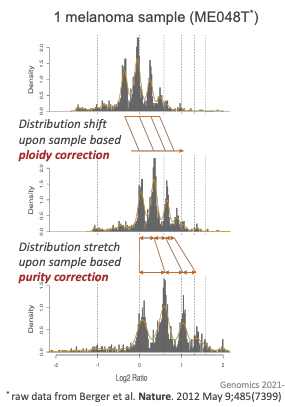
\includegraphics[width=0.6\textwidth]{image7}
  \label{fig: melanoma sample}
\end{figure}

In the figure we are looking at one tumor sample: a whole genome sequencing of
one melanoma sample \ref*{fig: melanoma sample}.

We see multiple peaks which correspond to different copy number states.

Let's suppose we have a genome with a backbone of three copies but we sequence a
bulk and we don't have 100\% purity but 80\% (so 20\% is contamination).

\begin{itemize}
  \item \emph{\textbf{Ploidy correction}}

  Computationally we assess the ploidy through the copy number space and then
  correct the data.
  
  From the tumor and the normal we obtain something like the first graph, and we
  could wrongly assume that the main peak is always in 0 (wild-type state of the
  genome), but it shouldn't.
  
  In fact, if we assess the ploidy and overall we see a backbone state of three
  copies for our genome, then the main peak should be shifted toward three.
  
  So, the \emph{ploidy correction shifts the distribution} towards the right
  (second graph).

  \item \emph{\textbf{Purity correction}}

  We correct our data and the \emph{{purity correction causes a stretch between
  the peaks}}, since tumor admixture dilutes the signal. So, the effect of purity
  correction is a wider spread between the peaks (third graph).
\end{itemize}

\begin{itemize}
\item
  If we have one extra copy in our tumor, the log2 ratio will be around 0.58 and
  so we would expect that the signal will peak around that value; for two extra
  copies we'd expect a peak around 1 and so on.
\item
  We'll have the peak of the normal state around 0 and then if we have an
  underrepresented allele in our tumor we'd get another peak around -1 for the
  hemizygous deletion and then the homozygous deletion.
\item
  If our signal is not 100\% pure tumor (so diluted by normal cells), the peak
  at -1 and 0.5 would be closer to the 0 peak for uncorrected data.
\end{itemize}

\emph{{When we correct for tumor purity we stretch the distribution to go to the
correct positions.}}

E.g.: 25 whole genome sequencing of melanoma samples

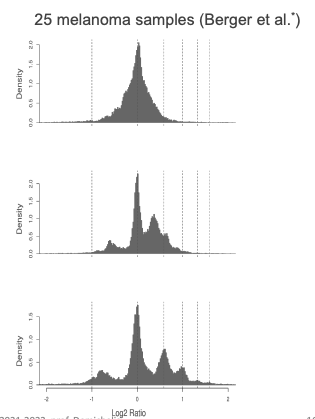
\includegraphics[width=3.42917in,height=4.56111in]{image8.png}\\

\begin{itemize}
\item
  1\textsuperscript{st} graph: The distribution of the log2 data of uncorrected
  signal, every melanoma sample is highly aberrant with a ploidy that is
  different between different individuals and a purity that is also different
  between different individuals. But we do have the tumor ploidy and purity so
  we can correct the data.
\item
  2\textsuperscript{nd} graph: we correct for ploidy
\item
  3\textsuperscript{rd} graph: we correct for purity too
\end{itemize}

If we don't correct our data we'll see much noise (as in the first graph).

From the corrected data we learn that:

\begin{itemize}
\item
  A lot of tumors have a backbone ploidy of two
\item
  There are some hemyzigous deletion not perfectly centered in one but closer to
  one in the 3\textsuperscript{rd} graph if compared to the
  1\textsuperscript{st}
\item
  Some signal is compatible with homozygous deletion
\item
  Whave a reasonable amount of signal for three copies which could come from a
  threeploid status of some tumors.
\end{itemize}

These corrections are part of standard preprocessing.

\emph{\textbf{Tumor Ploidy and Purity adjustment, corrected TCGA data}}

\emph{How commonly does suboptimal tumor purity affect proper copy number data
analysis?}

\emph{How common it is that purity is not equal to 100\% and ploidy is not equal
to 2 in any primary disease}

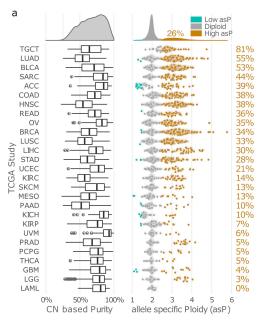
\includegraphics[width=3.24375in,height=3.97569in]{image9.png}\\

In the figure we can see a list of tumor types, where every draw is a tumor type
(lung carcinoma, bladder cancer, colon cancer, ovarian ecc.). On the x axis we
have tumor purity (1-admixture) going from 0 to 100\% and for each type we can
see the distribution of the tumor purity analysis of all the samples from the
TCGA dataset.

Every tumor type has a different number of sample profile

Looking at the GBM (glioblastoma multiforme), the middle vertical line is the
median signal of the distribution, there are outliers shown and the black
horizontal line represents the interquartile range.

Altogether across 27 tumor types they were able to assess the tumor cellularity,
clonality and all in about five thousand of those, meaning that a great fraction
of those had some optimal data (very strict criteria)

\begin{itemize}
\item
  The majority of the median distributions are above 50 \%.
\item
  The overall tumor cellularity was almost 70\%.
\end{itemize}

\emph{If we look at ploidy: what is the fraction within each tumor type with a
ploidy significantly above two}?

In the graph they are sorted by decreasing percentage of tumors with a ploidy
higher than two; for example, for the first and second tumor type, more than 50
\% of the primary tumors have a ploidy status above two so either they underwent
whole genome duplication (4 or more copies) or at least we have three.

Then we have some tumors with very low ploidy (blue dots) where at least one
copy of the entire genome is completely lost -\textgreater{} low allele specific
ploidy assessment.

The figure shows what happens to data when we correct for ploidy and purity

\begin{itemize}
\item
  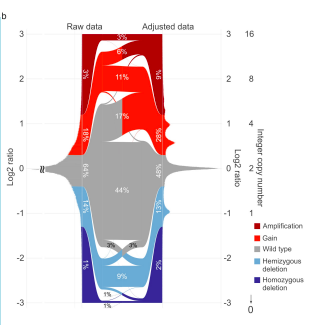
\includegraphics[width=3.65972in,height=3.76389in]{image10.png}\\
  On the y axis
  we have the log2 ratio
\item
  On the left side we have the raw data
\item
  On the right side the adjusted data
\end{itemize}

We can see where correction for ploidy and purity takes the signal.

Focusing just on the first half we can see that

we have the same noise we've seen for the melanoma uncorrected data.

\emph{The correction of the data results in the reclassification of 30\% of the
totality of the segments} (if we don't correct we have a wrong copy number
classification in 30\% of the cases)

Then there are certain copy numbers which are more or less affected by these
corrections.

What's interesting is that the correction led to the doubling of the homozygous
deletions that we were able to observe (these are very important because it
means that the proteic product won't be there at all).

\textbf{ALLELE SPECIFIC ANALYSIS (CNA, CNB SPACE)}

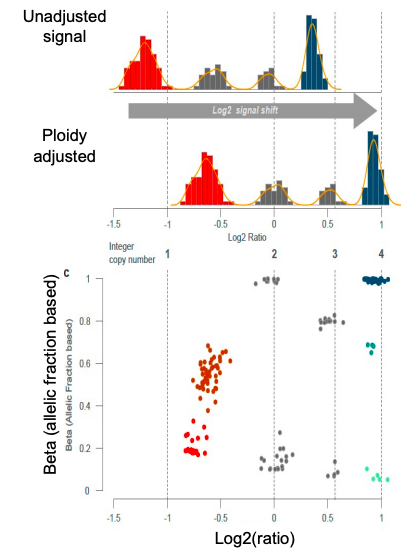
\includegraphics[width=3.12639in,height=4.35903in]{image11.png}\\

Thinking in terms of allele specific data:

\begin{enumerate}
\def\labelenumi{\arabic{enumi}.}
\item
  We have unadjusted signal
\item
  We adjust
\item
  Then we can go to the beta-log2 ratio space where we can see that the data
  underneath the peaks are belonging to specific clusters
\end{enumerate}

This suggests that by only looking at the log2 ratio we are unable to
distinguish the presence of clusters with different clonalities.

The most interesting information is the lower cluster (on the x=0 axis):

\begin{itemize}
\item
  Even when the T/N = 1 (tumor/normal ratio) what we can have is a status of one
  copy and one copy or something that equally gives a log2 ratio equal to 0 but
  which still represents copy neutral loss of heterozygosity (CN-LOH), so two
  copies on one allele and zero copies on the other.
\end{itemize}

+ example figures (will be added soon, I have to draw them)

1\textsuperscript{st} figure:

We have the loss of an allele on A so we'll have 2-1-2 copies

2\textsuperscript{nd} figure:

We have the same situation on allele A but allele B is doubled so we'll have
3-2-3 copies

So, in this situation, the gene x will have two copies but both of them coming
from the same allele (B).

Computing the log2 ratio in this situation we'll have the log2(2/2) which will
lead to the collocation on the 0 axis but on the lower part (due to the
clonality).

The log2-beta statuses allows us to distinguish the copy-neutral LOH.

Also for the gain is the same (three copies from the same allele and zero from
the other)

There are equations that allows us to go from here to a space where our
coordinates are the number of copies of allele A and number of copies of allele
B.\\
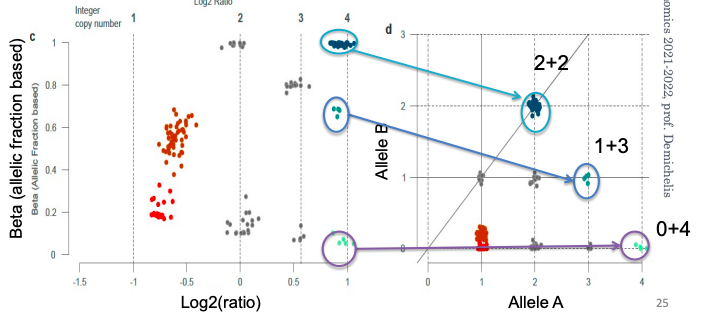
\includegraphics[width=6.68889in,height=2.97633in]{image12.png}\\
For four copies
we can have different combinations:

\begin{itemize}
\item
  2 copies of A + 2 copies of B,
\item
  3 copies of A + 1 copy of B
\item
  4 copies of A + 0 copies of B
\end{itemize}

The equations are not important, what's important is that once we have corrected
the data then we can shift our analysis up to the level of number of copies of
each allele for each gene.

\emph{Why is this important?}

E.g.: Let's imagine that for gene X we have one copy lost on allele A and a
point mutation on the allele B which leads to unfunctional product so full loss
of the protein.

If we instead are in the second case and the point mutation happened after the
duplication then we'll still have an allele functioning, whereas if it happened
before the duplication, we'd have again full loss of functional protein.

If we are able to distinguish the alleles we are able to also distinguish in
which situation we are (which means we can distinguish between what's functional
and what's not).

\begin{itemize}
\item
  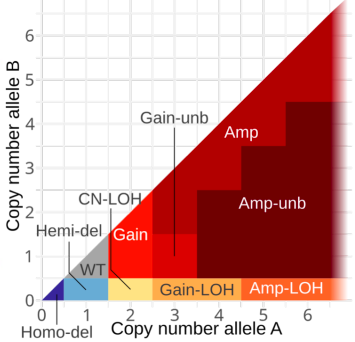
\includegraphics[width=3.00903in,height=2.89861in]{image13.png}\\
  Extra graph
  with the same space allele a/ allele B where we can divide the space in terms
  of total number of copies and also what happens on both.
\end{itemize}

So, this whole computation allows us:

\begin{itemize}
\item
  To reclassificate copy number status in the space by shifting and stretching
\item
  To also assign a copy number A and B to every segment of the genome, which
  means to every gene
\end{itemize}

If we do that we can see that many of the segments that have a total number of
copies equal to two are in fact 2+0 and not 1+1. This means that there is a
significant fraction of the genome which is apparently wild-type but which
actually underwent loss from one an allele and a gain on the other. This event
is called copy-neutral loss of heterozygosity (CN-LOH).

Copy-neutral because the number of copies doesn't change but there's been loss
of heterozygosity.

From the TCGA data, they observed a relevant fraction of high copy number levels
(4-5 copies) which all came from the same allele (one allele was lost and the
other underwent multiple cycles of duplication).

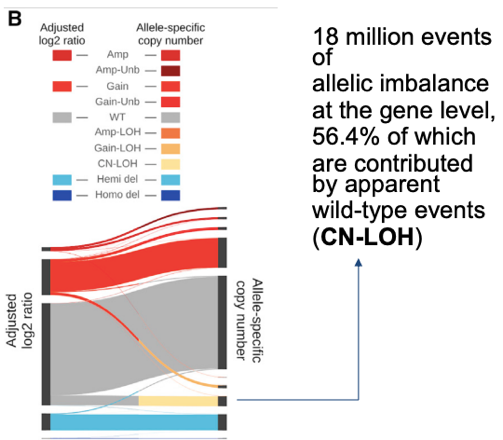
\includegraphics[width=2.29167in,height=2.00347in]{image14.png}\\

So, looking at
the copy number only we'd say there's a gain (which is true) but we wouldn't
have all the complete information (we also have to perform the allele analysis).

These information are relevant in precision medicine because there are ways to
target genes exploiting loss of heterozygosity and up until now it was only used
for deletions but now that's known, even if we have an apparent CN-LOH or we
have a copy number gain LOH we can still consider to use the same approach.

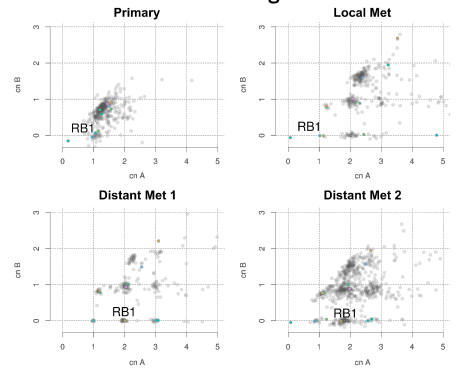
\includegraphics[width=6.58333in,height=5.0625in]{image15.png}\textbf{Case study
-- CNA, CNB real data example with multi-sample data from the same patient}\\

We have one patient and we're looking at a primary sample, for which we plot the
whole sequencing data in the copy number allele space and what we see (from the
first plot) is that:

\begin{itemize}
\item
  There's a cloud of dots (every dot is a gene) which has a total number of
  copies around two
\item
  There's a cluster that underwent hemyzygous deletion so we only have one copy
  of all the genes in there
\item
  There's one gene with a homozygous deletion (0,0).
\end{itemize}

Then we have three other metastatic sites for which they had biopsies so that
they could run whole genome sequencing and perform the analysis of the data in
the same space.

We have a local metastasis and two distant mets.

What we see:

\begin{itemize}
\item
  In distant met 1 there's no homozygous deletion*
\item
  In both the distant mets the gene RB1 gained an extra copy on allele A
\item
  In all the mets there are extra gains of copies of all the genes (maybe
  there's been a whole genome duplication of some sort)
\item
  In distant met 1 the data are as clean as to allow us to state that the data
  point in yellow/grey over the 1 is subclonal (if we have genes with 1+1 copy
  is equivalent to say it's a subclonal hemizygous loss, it means that all the
  cells have at least one copy and then some cells also have a second copy)
\item
  In terms of evolution, very likely extra copies of the whole genome also in
  the local met after the loss of the second copy of the gene
\item
  CN-LOH of many genes, including RB1
\item
  Level of subclonality overall not high
\end{itemize}

*\emph{How's possible that there's a homozygous deletion in the primary tumor
which is then absent in the distant mets?} No DNA can be regained, it's
impossible that the gene is reacquired, so probably the seeding of the distant
mets happened before the loss of the gene.

Another way to track evolution is to have \emph{serial time points.}

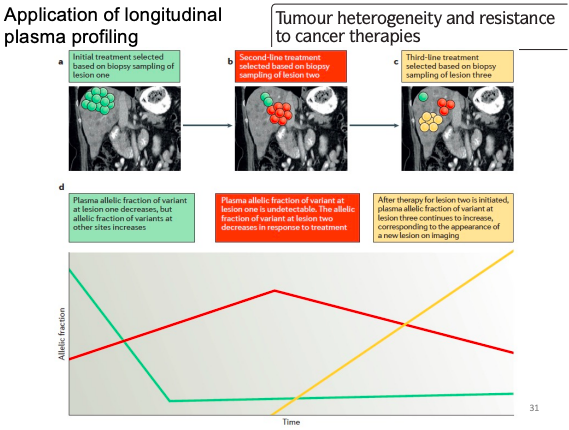
\includegraphics[width=6.68889in,height=5.05486in]{image16.png}\\

If we deal with biopsies over time we can track the evolution using the allelic
fraction of a lesion.

E.g.: reasoning in terms of point mutations, let's say we have a point mutation
at time point 0 in certain allelic fractions, which correspond to different
subsets, we track the fractions over time.

Doing this we can make inference of which subsets appear during the treatment
and are taking over (red one in the example figure).

Allelic fraction at any time point needs to be corrected for tumor content,
otherwise we would not be able to compare multiple time points from the same
patient.
